\chapter{Développement d'un système de \textit{plugins} entrées/sorties}

\section{Définition de la mission}
\subsection{Contexte}
Dès le début du développement de Vahana VR, la question des entrées et des sorties
du logiciel s'était posée. En effet, Studio étant un logiciel de montage de vidéos
360, ses seules entrées sont des fichiers vidéos, issus des caméras de la monture. De même, la seule sortie
est le fichier vidéo 360, comme présenté dans la section \cf{exportation}.\\
Ce qui est ici appelé \emph{entrées} sont les données envoyées au programme, quand
les \emph{sorties} sont les données émises par ce programme en retour.\\
Pour permettre la vidéo 360 en direct, Vahana VR, contrairement à Studio, s'affranchit des fichiers
vidéos importés et propose de capturer directement les images des caméras, via
des cartes d'acquisitions branchées sur la machine utilisée. De même, Vahana VR peut émettre 
plusieurs fluxs en sortie permettant, par exemple, le \textit{streaming} ou la réémissions vers
une carte d'acquisition, en plus de l'export de la vidéo 360 sur le disque dur.\\
\begin{figure}
  \centering
  \setlength{\unitlength}{8mm}
  \begin{picture}(16,5)
    \linethickness{0.3mm}
    \thicklines
    \put(4,0.5){\small Entrées}
    \put(4,4.2){\vector(2,-1){2}} \put(2.2,4.2){$1$ audio }
    \put(4,3){\vector(2,0){2}}    \put(2,2.3){$n$ vidéos}
    \put(4,1.8){\vector(2,1){2}}  \put(4.1,2.2){$\Shortstack{. . . .}$}
    \put(7,0.5){\small Stitch 360}
    \put(6,2){\framebox(4,2){\large Vahana VR}}
    \put(11,0.5){\small Sorties}
    \put(10,3){\vector(3,2){2}}  \put(12.25,4.2){HDMI}
    \put(10,3){\vector(4,1){2}}  \put(12.25,3.4){SDI}
    \put(10,3){\vector(4,-1){2}} \put(12.25,2.4){RTMP}
    \put(10,3){\vector(3,-2){2}} \put(12.25,1.6){Disque dur}
  \end{picture}
  \caption{Schéma des entrées/sorties de Vahana VR}
\end{figure}

\subsection{Problématique}
Dès lors, Vahana VR étant destiné à des sociétés de production, il doit
être compatible avec un maximum de standards, caméras et cartes d'acquisitions vidéos
pour être facilement adopté. Cependant, tout matériel informatique requérant des pilotes
\footnote{Programme permettant au système d'exploitation d'interagir avec le matériel couvert par ce pilote\cite{pilote-informatique}.}
, et, les besoins des clients en entrées/sorties n'étant pas les mêmes, il n'était
alors pas possible de concevoir un logiciel monolithique contenant tous les programmes 
d'entrées/sorties supportés~: l'installation de Vahana VR aurait requis au client 
une installation de l'ensemble des pilotes.\\
De plus, un client pourrait souhaiter utiliser du matériel entrée/sortie encore
non supporté. Il serait intéressant qu'il puisse réaliser son propre développement
dans l'écosystème de Vahana VR; ainsi le logiciel pourrait devenir virtuellement
compatible avec n'importe quel standard, caméra ou carte d'acquisition.\\
Il fallait donc développer un système assurant à la fois la compatibilité
entre Vahana VR et ces matériels, et intégrant les contraintes exposées.\\

\subsection{Objectifs}
Au début de ce stage, une solution avait déjà été esquissée et était déjà en partie
mise à l'\oe uvre. Cependant un certain travail de développement était encore nécessaire.\\
\newline
Les objectifs retenus pour cette mission ont donc été~:
\begin{itemize}
  \item Développer les entrées HDMI\footnote{\textit{High Definition Multimedia Interface}, 
  norme de diffusion audio/vidéo numérique\cite{hdmi}.} et SDI\footnote{\textit{Serial Digital Interface}, 
  protocole de diffusion vidéo numérique\cite{sdi}.}.
  \item Développer les sorties HDMI et SDI.
  \item Développer des entrées/sorties Ethernet et PCIe\footnote{\textit{PCI Express}, standard
  de connexion de cartes d'extension sur la carte mère d'un ordinateur\cite{pci-express}.}
  spécifiques, à la demande d'un client.
  \item Déployer l'ensemble des \textit{plugins} sur un dépôt séparé.
  \item Documenter et vérifier la bonne intégration des \textit{plugins} dans Vahana VR.
\end{itemize}

\begin{figure}
  \centering
  \begin{minipage}{0.2\textwidth}
    \centering
    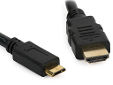
\includegraphics[width=3cm]{images/hdmi-cable.jpg}
    \captionof{subfigure}{HDMI}
  \end{minipage}%
  \hspace{0.03\textwidth}
  \begin{minipage}{0.2\textwidth}
    \centering
    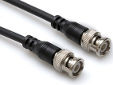
\includegraphics[width=3cm]{images/sdi-cable.jpg}
    \captionof{subfigure}{SDI}
  \end{minipage}%
  \hspace{0.03\textwidth}
  \begin{minipage}{0.2\textwidth}
    \centering
    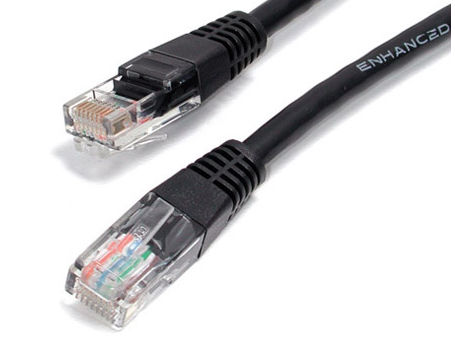
\includegraphics[width=3cm]{images/ethernet-cable.jpg}
    \captionof{subfigure}{Ethernet}
  \end{minipage}%
  \hspace{0.03\textwidth}
  \begin{minipage}{0.2\textwidth}
    \centering
    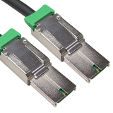
\includegraphics[width=3cm]{images/pcie-cable.jpg}
    \captionof{subfigure}{PCIe}
  \end{minipage}
  \caption{Illustration des différents connecteurs utilisées par Vahana VR}
\end{figure}


\section{Réalisation}
\subsection{Architecture de la solution}
Il s'agissait tout d'abord de saisir le concept de la Programmation Orientée Composant, et la manière
dont il est appliqué pour Vahana VR.\\
Cette approche propose d'utiliser différents \emph{composants}
qui vont interagir entre eux~: ici les \textit{plugins} entrées/sorties avec Vahana VR. On entend
par composants, ou \textit{plugins}, des bibliothèques (fichiers .dll) qui peuvent être chargées et utilisées
par un programme client, ici Vahana VR. Tout comme les dépendances\footnote{Présentées dans 
la section \cf{integration-dependances-player}.}, un composant va fournir un ensemble
de fonctions, déclarées dans les \textit{headers} qui accompagnent ces
bibliothèques. Ces fonctions sont donc regroupées dans un module externe
au logiciel qui peut y faire appel si besoin, ou non.\cite{poc}\\
L'intérêt d'une telle approche est qu'elle permet d'introduire de la modularité dans 
l'architecture du projet, les \textit{plugins} peuvent être développés séparément du logiciel
client. Et surtout, ils peuvent être distribués séparément du logiciel ou être remplacés
au besoin sans remplacer tout le logiciel. Un composant peut également être réutilisé par d'autres programmes.\\
Enfin, si l'analogie avec les dépendances pouvait être faite jusqu'ici, contrairement à ces
dernières dont l'utilisation est réalisée \enquote{en dur} dans le code, un composant est
utilisé indirectement via ses interfaces. Car, c'est à son lancement que le programme charge les composants
\emph{dynamiquement} présents et qui respectent l'interface attendue, celle du
\textit{header} du composant~: le code de la bibliothèque est inconnu car compilé, seul sont
connues les fonctions attendues du composant.\cite{plugin}\\
Un exemple de \textit{plugins}, est typiquement les extensions d'un navigateur web. Ces composants
ont été écrits pour le navigateur, en répondant à une interface attendue par ce logiciel,
et peuvent être activés ou désactivés à volonté par l'utilisateur.\\
\newline
Concrètement, sont définie dans les \textit{headers} de Vahana VR toutes les interfaces.
Un \textit{plugin} pour Vahana VR peut implémenter trois interfaces~:
\begin{itemize}
  \item Une interface pour créer une entrée.
  \item Une interface pour créer une sortie.
  \item Une interface \textit{discovery} dont le rôle est d'indiquer les possibilités
    de créations entrées/sorties.
\end{itemize}
Ainsi, lors de son exécution, Vahana VR va chercher les bibliothèques présents dans le dossier
\mintinline{shell-session}{plugins} à sa racine et va charger les \textit{plugins} implémentant
au moins un de ces interfaces. Le logiciel possède désormais une collection d'entrées
ou de sorties potentielles. En fonction de données renvoyée par les \textit{discovery},
l'utilisateur peut demander, dans l'interface de Vahana VR, de 
créer une nouvelle entrée -- ou sortie -- pour tel \textit{plugin}. Et via les
interface implémentées par le \textit{plugin}, le logiciel va pouvoir faire exécuter le code
du \textit{plugin} de création de l'entrée -- ou sortie --.\\

\subsection{Conception des \textit{plugins}}
\subsubsection{Prise en main}
Cinq plugins furent écrits et maintenus durant ce stage. L'approche retenue fut de créer
un nouveau plugin par constructeur. Ces plugins s'appuient en effet sur du matériel
externe à VideoStitch, comme des caméras ou des cartes d'acquisition. Les plugins
développés sont les suivant~:
\begin{itemize}
  \item Plugin d'entrée/sortie SDI pour les cartes d'acquisition DeckLink
  \footnote{\url{https://www.blackmagicdesign.com/fr/products/decklink/models}}.
  \item Plugin d'entrée HDMI pour les cartes d'acquisition Yuan
  \footnote{\url{https://www.blackmagicdesign.com/fr/products/decklink/models}}.
  \item Plugin d'entrée HDMI pour les cartes d'acquisition Magewell
  \footnote{\url{https://www.blackmagicdesign.com/fr/products/decklink/models}}.
  \item Plugin d'entrée PCIe pour les caméras xiB de Ximea
  \footnote{\url{http://www.ximea.com/en/products/application-specific-oem-and-custom-cameras/pci-express-high-speed-cameras}}.
  \item Plugin d'entrée GigE\footnote{Standard pour les caméras industrielle utilisant 
  la transmission par Ethernet\cite{gige}.} pour les caméras Genie TS de Teledyne Dalsa\footnote{\url{http://www.teledynedalsa.com/imaging/products/cameras/area-scan/genie-ts/}}.
\end{itemize}
Les trois premiers plugins proposent une acquisition pour des normes standard, HMDI et SDI, 
et permettent d'utiliser n'importe quelle caméra compatible avec ces standards, quand les
deux restant proposent une capture pour des caméras d'un constructeur en particulier.
Les premiers plugins sont systématiquement distribués avec Vahana VR. Les deux derniers
furent développé à la demande d'un client et ne sont distribués selon les besoins.\\
\newline
Leurs développements ont suivis relativement les même étapes.
Tout d'abord, il s'agissait d'installer la caméra ou la carte d'acquisition sur la 
machine de développement et de la mettre en fonctionnement. Le constructeur va fournir
deux ressources~: le pilote pour que le système puisse utiliser le matériel, et un
SDK pour qu'un développeur puisse développer une application utilisant ce matériel.
La figure~\ref{entree-sortie-schema} résume les interactions de Vahana au matériel d'entrée/sortie.
\begin{figure}
  \centering
  \setlength{\unitlength}{8mm}
  \begin{picture}(5,8)
    \linethickness{0.3mm}
    \thicklines
    \put(1,8){\framebox(3,1){Vahana VR}}        \put(2,8){\vector(0,-1){1}} \put(3,7){\vector(0,1){1}}
    \put(1,6){\framebox(3,1){\textit{Plugin}}}  \put(2,6){\vector(0,-1){1}} \put(3,5){\vector(0,1){1}}
    \put(1,4){\framebox(3,1){SDK constructeur}} \put(2,4){\vector(0,-1){1}} \put(3,3){\vector(0,1){1}}
    \put(1,2){\framebox(3,1){Driver}}           \put(2,2){\vector(0,-1){1}} \put(3,1){\vector(0,1){1}}
    \put(1,0){\framebox(3,1){Matériel}}
  \end{picture}
  \caption{Schéma des interactions de Vahana VR au matériel d'entrée/sorties}
  \label{entree-sortie-schema}
\end{figure}
Le plugin développé correspond au patron de conception\footnote{Ou \textit{design pattern},
qui est une bonne pratique de conception logicielle.} \emph{adaptateur}, c'est-à-dire qu'il convertit les interfaces
et le fonctionnement du SDK du constructeur sous une autre interface, celle attendue
par le programme client, Vahana VR\cite{adapter-design-pattern}.

\subsubsection{Implémentations}
Ces interfaces attendues sont définies dans Vahana, et développer un plugin consiste
à en réaliser les implémentations~: ce fut la seconde partie du développement.\\
Tous les plugins développés implémentent l'interface \cppinline{Input}. Quelques fonctions recquiert 
de l'attention~:
\begin{itemize}
  \item \cppinline{Input* create(const Config* parameters)} : appellée si \cppinline{handle}
  a réussi, cette fonction tente la création de l'entrée avec les paramètres donnés
  et renvoie un pointeur sur l'objet \cppinline{Input} créé, si cela a réussi, sinon
  un pointeur nul.
  \item \cppinline{std::string name()} : permet de distinguer les plugins entre eux (en
  effet, ils partagent tous la même interface), pour appeller la fonction \cppinline{create} 
  du bon plugin.
  \item \cppinline{bool readFrame(uint32_t* video)} : appellée par Vahana VR, le plugin doit renvoyer la
  dernière image capturée par la caméra -- ou carte d'acquisition. Cette fonction
  est appellée au moins 25 fois par seconde, une vidéo n'étant finalement 
  qu'une succession très rapide d'images.\\
  L'image doit être renvoyée dans le format de couleur RGBA.
\end{itemize}
La création d'un \cppinline{Input} réclame quelques paramètres, qui sont envoyés 
au travers de l'argument \cppinline{parameters}. Cette configuration demandée par
l'utilisateur contient, par exemple, quelle caméra utiliser,
la résolution de l'image capturée (largeur et hauteur en pixel) ou encore le nombre d'images
par seconde qui seront capturées (règle le nombre d'appels de Vahana VR à la fonction \cppinline{readFrame}). 
Cette liste est enrichie de divers paramètres selon le plugin, et les capacités du SDK du constructeur.\\
L'implémentation de l'interface \cppinline{Output} est similaire à l'interface \cppinline{Input},
à la différence qu'elle envoie des images, avec la méthode \cppinline{writeFrame}, et ne les lit pas (méthode \cppinline{readFrame}).\\
\newline
L'interface \cppinline{Discovery} permet d'indiquer à Vahana VR, et par extension
à l'utilisateur, les ensembles de de paramètres et valeurs utilisables pour le plugin. 
L'implémentation de cette interface s'effectue sur quelques fonctions~:
\begin{itemize}
  \item \cppinline{std::string name()} : tout comme \cppinline{Input}, permet de distinguer les plugins entre eux.
  \item \cppinline{std::vector<Device> devices()} : indique la liste des entrées/sorties
  disponibles; un \cppinline{Device} est simplement
  \item \cppinline{std::vector<DisplayMode> supportedVideoModes(const Plugin::Device& device)}
\end{itemize}

\subsection{Quelques difficultés et solutions spécifiques}
Chaque plugin s'appuyant sur un SDK d'un constructeur différent, un certain nombre
de problèmes furent rencontrés pour réaliser l'implémentation totale des interfaces.
Quelques difficultés et leurs solutions sont notables.\\

\subsubsection{Partage des ressources Yuan}

\subsubsection{Augmentation des interfaces DeckLink}

\subsubsection{Lecture des images Ximea}


\section{Déploiement}
\subsection{Création du dépôt VideoStitch-IO}
Les \textit{plugins} étaient à l'origine développés dans le dépôt VideoStitch-apps. Il faisait
cependant plus sens qu'ils soient déplacés dans un dépôt distinct, car étant relativement indépendant
de Vahana VR. Cette opération nécessitait, comme dans la section \cf{integration-apps}, un déplacement du dossier
de développement et de l'historique des modifications. La technique présentée en annexe~
\ref{deplacer-historique-depots} (p.\pageref{deplacer-historique-depots}) fut de
nouveau utilisée avec succès, déplaçant le contenu du dossier \mintinline{shell-session}{src/plugins/}
du dépôt VideoStitch-apps vers le dossier \mintinline{shell-session}{src/} sur le dépôt VideoStitch-IO.\\
\newline
Ce nouveau dépôt a été organisé de manière sensiblement équivalente à celui de VideoStitch-apps, 
cependant la chaîne de compilation des \textit{plugins} fut mise à jour pour prendre en compte
cette nouvelle organisation.\\
En outre, ce dépôt nécessitait, tout comme VideoStitch-apps, du VideoStitch-SDK et des dépendances
pour être compilé. Le script \mintinline{shell-session}{update.sh}\footnote{Voir la section \cf{integration-apps}.}
fut alors partagé, et les \textit{plugins} purent être compilés à nouveau.\\
\newline
Le Buildbot fut alors mis à jour également d'un nouveau builder prenant en charge ce dépôt.
Une liste d'étapes similaires au listing~\ref{windows-apps} (p.\pageref{windows-apps}) furent écrites pour
compiler automatiquement les \textit{plugins} et les mettre à disposition sur une page de 
téléchargement interne.\\
Le script \mintinline{shell-session}{update.sh} a alors été augmenté pour télécharger
la dernière version des \textit{plugins} et les copier dans la copie du dépôt VideoStitch-apps
du développeur appelant le script. Les \textit{plugins} ont été déplacés sur un autre dépôt
mais sont toujours nécessaires pour générer utiliser Vahana VR avec toutes ses
capacités.\\
Enfin, les plugins DeckLink, Magewell et Yuan furent ajoutés à l'installateur de Vahana VR, 
permettant de couvrir les besoins usuels du logiciel.

\subsection{Documentation}
Deux documentations ont ensuite été écrites.\\
Chaque plugin fut
Puis une documentation générale fut écrite sur le wiki interne. 

\subsection{Tests et \textit{QA} de l'intégration des \textit{plugins}}


\section{Bilan et suite}

